
It originates in \fullcite{scvo85} (1985). 

 
In Remark 9 (p.29) of \textcite{aubb17} (2017) we find: 
\begin{displayquote}
{\color{darkgray}
We also remark that the discontinuous
pressure version of the Hood–Taylor element typically
results in an unstable method. However, stability can be
recovered by imposing certain restrictions on the mesh for
$k \ge 3$ (see \cite{voge83}; \cite{scvo85}), or
by taking advantage of suitable stabilization procedures for
$k\ge 1$ (see Mansfield, 1982; Boffi, 1995).
}
\end{displayquote}

In \textcite{fams21} (2021) we find:
\begin{displayquote}
{\color{darkgray}
The Scott-Vogelius element is given by choosing continuous piecewise 
polynomials of degree $k$ for the velocity and discontinuous piecewise 
polynomials of degree $k-1$ for the pressure. While this clearly
implies that $\nabla\cdot V_h \in Q_h$, inf-sup stability of the 
Scott–Vogelius element is more delicate, and is a topic of ongoing research. 
In two dimensions, Scott \& Vogelius proved \cite{scvo85} that the element is inf-sup
stable for $k\ge 4$ if the mesh does not have nearly singular vertices. 
In three dimensions, it was proven more recently in \cite{zhan11b} 
that the element is stable for $k\ge 6$ on uniform meshes. The stability on general
tetrahedral meshes continues to be an open question.

On barycentrically refined meshes, however, the pair is known to 
be stable for polynomial order
$k = d$, see [48, Section 4.6] for the 2D case and 
\cite{zhan05} for the 3D case. If one is willing to 
consider the more complicated Powell–Sabin split, the order 
can be reduced further to $k=d-1$ \cite{zhan08,zhan11a}. The two
refinement patterns are shown for the two dimensional case 
in Figure 1 [see below]. In this work we will consider
the case of $k \ge d$ on barycentrically refined meshes, but 
the arguments apply mutatis mutandis to the Powell–Sabin split.
}
\end{displayquote}

\begin{center}
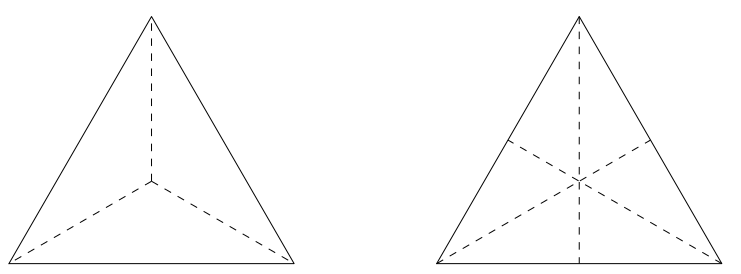
\includegraphics[width=9cm]{images/pair_scott_vogelius/scottvogelius_split}\\
{\captionfont 
Barycentrically refined triangle (also known as Alfeld split) on the left,
and Powell–Sabin split on the right.\\ Taken from \textcite{fams21} (2021).}
\end{center}

\textcite{cael11} (2011) state:
\begin{displayquote}
{\color{darkgray}
The SV element pair is not yet very well known,
and so we now give a brief description of it. In essence, the SV pair is the same as
the Taylor-Hood pair except that the pressure space is discontinuous and either
(i) for $k \ge d$, the mesh is a barycenter refinement of a regular mesh, or
(ii) for $k = 2, d = 3$, the mesh is formed from a barycenter refined mesh by
connecting the barycenter nodes (i.e., a Powell–Sabin tetrahedralization).
In short, polynomials of degree $k$ and $k-1$ are used to approximate the velocity
and pressure spaces, respectively, and the mesh ${\cal T}_h$ that is used must be derived from
a regular triangulation (tetrahedralization) of $\Omega$, where each element is refined as
stated above. With these mesh constructions, it was proved by Zhang in [42, 44] that
the SV elements are LBB stable, and, consequently, also have optimal approximation
properties. It is well known that the TH pair is LBB stable and admits optimal
approximation properties for these cases as well [9]. We will restrict our definition of
SV elements to these cases where they are LBB stable.
}
\end{displayquote}



See also \textcite{jolm17} (2017) in which the $P_2\times P_1$, Scott-Vogelius ($P_2\times P_{-1}$), 
Bernardi-Raugel, and $P_2^+\times P_{-1}$ elements 
are compared for a thermo-mechanically driven convection problem in a triangle (see \stone~51, 
although I use the $P_1^+\times P_1$ element in this stone).


\begin{center}
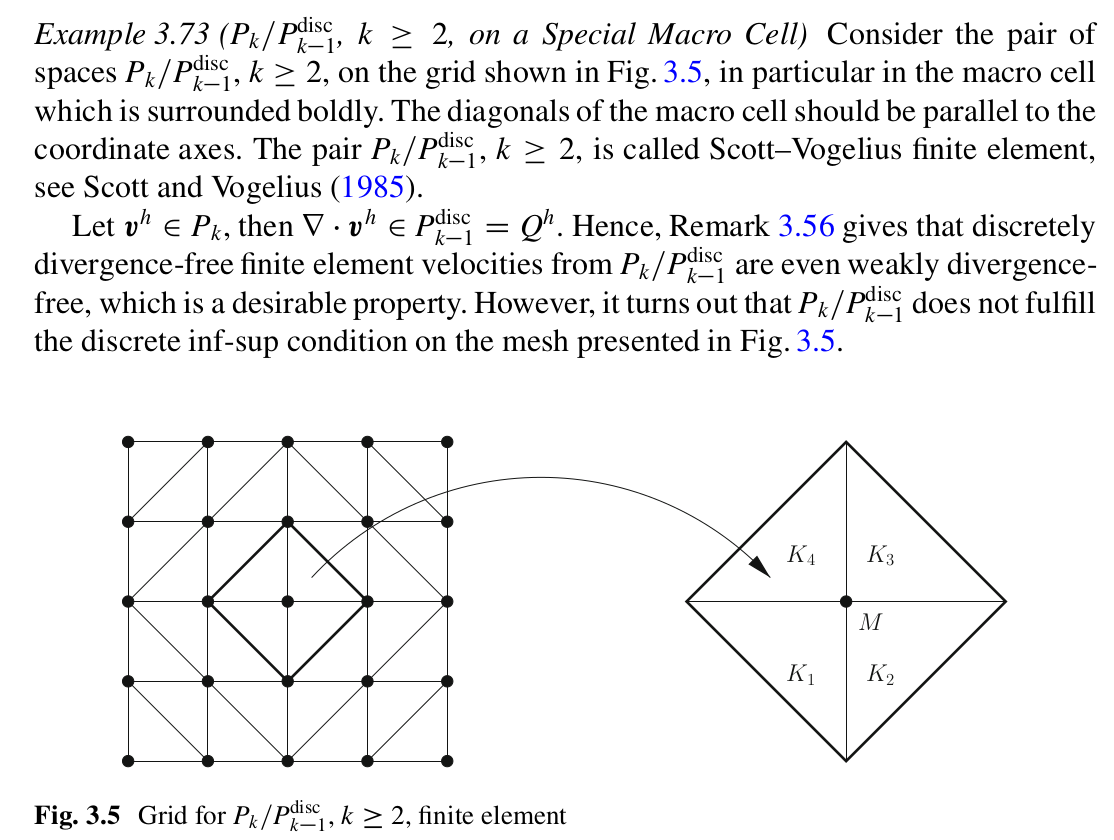
\includegraphics[width=10cm]{images/pair_scott_vogelius/john_scott_vogelius}\\
\captionfont{Taken from John \cite[p70]{john16}.} 
\end{center}


In \textcite{befh21} (2021) this element is used in its $(P_3)^2-P_2^{\text{disc}}$ form.

\begin{center}
\url{https://defelement.com/elements/scott-vogelius.html}
\end{center}

